\chapter{Technology Review}
\label{cha:review}

\section*{Introduction of Technology Review}

This chapter provides a comprehensive review of the technologies, frameworks, and services employed in the development of ``\textit{Guardians of the Chess Grandmaster},'' a web-based chess training platform designed to challenge players and develop grandmaster-level thinking skills. The technology review demonstrates the research and evaluation conducted to select appropriate tools and approaches for building a modern, scalable, and performant web application.

As established in the introduction, the primary objectives of this project are to:
\begin{itemize}
    \item Provide an interactive chess training platform with puzzle-based learning
    \item Deliver real-time feedback on player moves and positions
    \item Track user progress and performance analytics
    \item Ensure responsive performance across desktop and mobile devices
    \item Maintain scalability for growing user base and puzzle database
\end{itemize}

To achieve these objectives, each technology selection was evaluated based on specific criteria relevant to chess training applications: real-time interactivity, data structure flexibility for chess positions, performance optimization for board rendering, and maintainability for ongoing development. This review examines technologies at a conceptual level, with justification based on project requirements, industry standards, and academic literature.

The review is structured to cover all major components of the technology stack:
\begin{itemize}
    \item Frontend technologies (React, TypeScript, Vite)
    \item Backend infrastructure (Node.js, Express.js)
    \item Database systems (MongoDB)
    \item Development standards (REST, JSON)
    \item Third-party libraries (Chess.js, React-Chessboard)
\end{itemize}

Each section examines the conceptual foundations of the technology, its key features, and the rationale for its selection in the context of building an effective chess training platform.

\section{Frontend Technologies}

The \texttt{frontend} is the primary interface between users and the system. For a chess training platform, \texttt{frontend} technology choices directly affect board responsiveness, piece movement smoothness, and the overall puzzle-solving experience.

\subsection*{React Framework}

React is a declarative, component-based JavaScript library developed by Meta for building user interfaces. Unlike full-stack frameworks such as Angular or Vue, React focuses on the view layer, giving developers architectural flexibility for other concerns \cite{gackenheimer2015react} (React Documentation: \href{https://react.dev/}{react.dev}).

React's architecture rests on three core concepts. First, \textbf{component-based architecture} allows applications to be built from modular, reusable components that encapsulate structure, styling, and behaviour. For a chess application, the board, individual pieces, move history panel, and puzzle instructions can each be isolated components. A \texttt{ChessBoard} component might contain 64 \texttt{Square} components, each potentially housing a \texttt{Piece} component and the coordinates (a-h, 1-8), as illustrated in Figure~\ref{fig:chessboard_setup}.

\begin{figure}[ht]
    \centering
    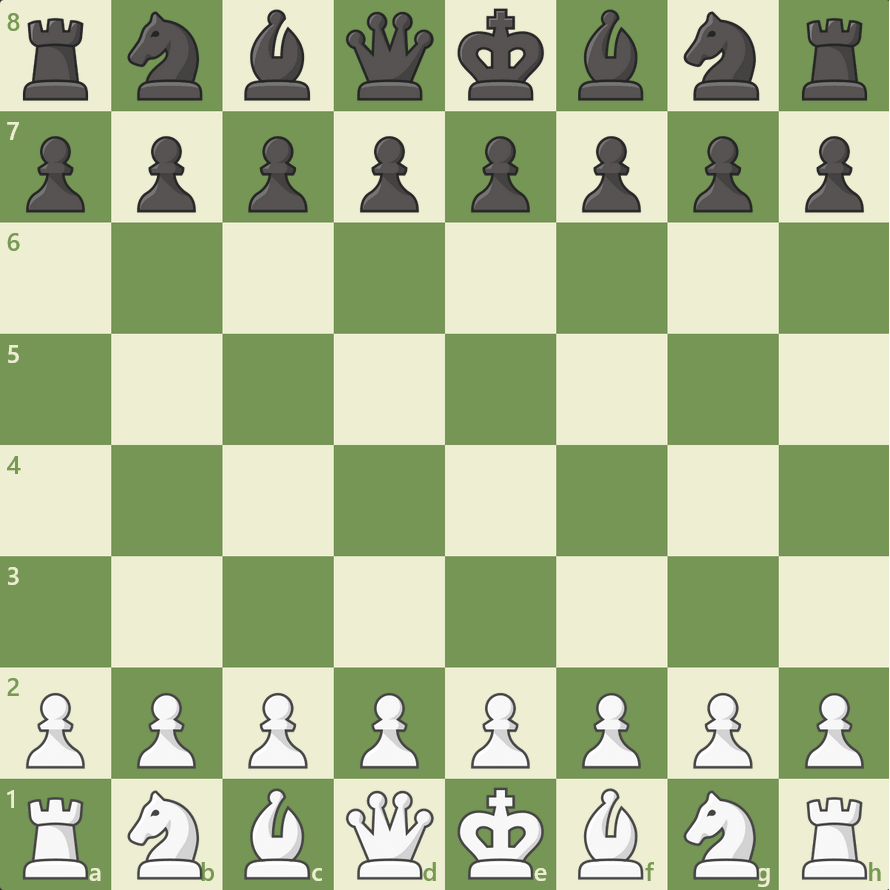
\includegraphics[width=0.5\linewidth]{images//Review_Image/Chessboard-Setup.png}
    \caption{Chess Board setup (Source: \href{https://www.chess.com/terms/chess}{Chess.com})}
    \label{fig:chessboard_setup}
\end{figure}

Second, React's \textbf{virtual DOM and reconciliation} mechanism avoids costly direct DOM manipulation. When state changes, React compares a new virtual DOM tree against the previous version and applies only the minimal set of real DOM updates \cite{aggarwal2018modern}. For a chess application where piece movements and board state changes occur frequently, this prevents unnecessary full re-renders and maintains smooth interactions.

Third, React enforces \textbf{unidirectional data flow}: data flows downward via props and state changes propagate upward through callbacks \cite{hunt2016react}. This predictability simplifies debugging and testing. When a user moves a piece, the event flows upward to the parent component managing game state, which validates the move via Chess.js, updates state, and propagates the new position down to child components for rendering.

React was selected for this project due to its performance for interactive applications \cite{aggarwal2018modern}, strong component reusability across training modes (tactical puzzles, endgame training, opening practice), its rich ecosystem (React Router, Context API, UI libraries), and its position as the most widely used web framework per the Stack Overflow Developer Survey 2023 \href{https://survey.stackoverflow.co/2023/}{(Stack Overflow, 2023)}. Critically, the chess-specific library React-Chessboard is built for React, enabling seamless integration.

\subsection*{TypeScript}

TypeScript is a statically-typed superset of JavaScript developed by Microsoft that adds optional type annotations and compiles to standard JavaScript \cite{bierman2014typescript} (TypeScript Documentation: \href{https://www.typescriptlang.org/docs/}{typescriptlang.org}).

TypeScript's \textbf{static type system} allows explicit declaration of variable types, function parameters, and return values, with the compiler catching mismatches before runtime. \textbf{Type inference} reduces verbose annotations while maintaining safety \href{https://www.typescriptlang.org/docs/handbook/}{(TypeScript Handbook)}, and \textbf{interfaces} define contracts for object shapes that serve simultaneously as type-checking mechanisms and inline documentation.

TypeScript was selected for several reasons relevant to this project. Research by Gao et al.\ \cite{gao2017type} found TypeScript detects approximately 15\% of bugs that would otherwise surface at runtime---a significant benefit for complex chess logic such as move validation, position evaluation, and rating calculations. TypeScript also provides superior IDE support with IntelliSense and autocomplete for chess.js library methods. For a project evolving over multiple months, its compile-time safety makes refactoring safer, and its type annotations enforce API contract consistency between \texttt{frontend} and \texttt{backend}.

\subsection*{Vite Build Tool}

Vite is a modern \texttt{frontend} build tool created by Evan You that prioritises developer experience through instant server startup and rapid hot module replacement \href{https://vitejs.dev/}{(Vite Documentation)}.

Traditional bundlers such as Webpack must bundle the entire application before the development server starts, becoming slow as codebases grow. Vite addresses this by serving source code as native ES modules during development---leveraging native browser ES module support \href{https://tc39.es/ecma262/}{(ECMAScript Modules)}---and only transforming files on-demand as the browser requests them. When source files change, Vite's HMR invalidates only the changed module, preserving application state and delivering near-instantaneous browser updates \href{https://vitejs.dev/guide/features.html}{(Vite Features)}. For production, Vite uses Rollup \href{https://rollupjs.org/}{(Rollup)} to apply tree-shaking, code splitting, and minification.

Vite was selected for its development velocity---iterating on chess puzzles and training modes benefits greatly from rapid feedback loops. Benchmarks show Vite achieving 10--100$\times$ faster cold server starts and 2--10$\times$ faster HMR compared to Webpack \cite{vite_comparison}. It also provides first-class support for React and TypeScript through official plugins, requiring no complex configuration.

\section{Backend Technologies}

The \texttt{backend} serves as the application's server-side logic layer, handling data processing, business rules, authentication, and database communication. For a chess training platform, \texttt{backend} requirements include puzzle delivery, move validation, user progress tracking, and rating calculations.

\subsection*{Node.js Runtime Environment}

Node.js is a JavaScript runtime built on Chrome's V8 engine, enabling JavaScript execution outside the browser. Created by Ryan Dahl in 2009, it brought JavaScript to server-side development, enabling full-stack JavaScript applications \href{https://nodejs.org/en/about/}{(About Node.js)}.

Node.js employs an \textbf{event-driven, non-blocking architecture} centred on an event loop \cite{tilkov2010nodejs}. Rather than spawning a new thread per connection, the single-threaded event loop accepts requests, delegates I/O operations to the system, continues processing other requests without blocking, and executes callbacks on completion. This allows Node.js to handle thousands of concurrent connections with minimal memory overhead, well-suited to the I/O-intensive nature of a chess training server \cite{chaniotis2015nodejs}. The V8 engine compiles JavaScript to native machine code \href{https://v8.dev/docs}{(V8 Docs)}, and the npm ecosystem provides access to over 2 million reusable packages \href{https://www.npmjs.com/}{(npm Registry)}.

Node.js was selected principally for \textbf{JavaScript uniformity}: using a single language across \texttt{frontend} and \texttt{backend} eliminates context switching and enables sharing of move validation logic, FEN parsing utilities, and notation converters between client and server \cite{pautasso2016rest}. It also handles JSON natively, simplifying data exchange between MongoDB and the React \texttt{frontend} \cite{nurseitov2009json}, and provides strong real-time capabilities for potential future features such as live multiplayer analysis and collaborative puzzle solving \cite{pimentel2012websockets}.

\subsection*{Express.js Framework}
Express.js is a minimal, unopinionated web framework for Node.js, first released in 2010 and now the de facto standard for Node.js web development \href{https://expressjs.com/}{(Express Documentation)}.

Express applications are composed of \textbf{middleware functions} with access to the request and response objects and the next function in the request-response cycle \cite{brown2014express}. Middleware can execute code, modify request/response objects, end the cycle by sending a response, or pass control to the next middleware---promoting modularity and code reuse. Its flexible \textbf{routing} supports HTTP method handlers, route parameters (e.g.\ \texttt{/puzzles/:id}), query parameters, and modular route grouping. Unlike opinionated frameworks such as Django or Rails, Express's minimalism allows developers to choose appropriate tools for specific requirements without working around framework constraints \cite{mardan2014express}.

Express was selected for its lightweight foundation, its natural fit with RESTful API design, and its extensive middleware ecosystem (e.g.\ \texttt{cors}, \texttt{helmet}, \texttt{morgan}, \texttt{express-rate-limit}). It is production-proven at scale, used by organisations including Uber and IBM \href{https://nodejs.org/en/about/case-studies/}{(Node.js Case Studies)}.

\section{Database Technologies}

\subsection*{MongoDB NoSQL Database}

MongoDB is a \textbf{document-oriented} NoSQL database that stores data in flexible, JSON-like documents called BSON (Binary JSON) \href{https://www.mongodb.com/docs/manual/}{MongoDB Manual}. Released in 2009, MongoDB represents a paradigm shift from traditional relational databases toward schema-flexible document storage.

\subsubsection*{Conceptual Foundation}

\textbf{Document Model} $\rightarrow$ Unlike relational databases that store data in tables with fixed schemas, MongoDB stores data in documents---self-contained data structures that can include nested objects and arrays \cite{chodorow2013mongodb}. A chess puzzle document might look like \ref{fig:mde}:

\begin{figure}
    \centering
    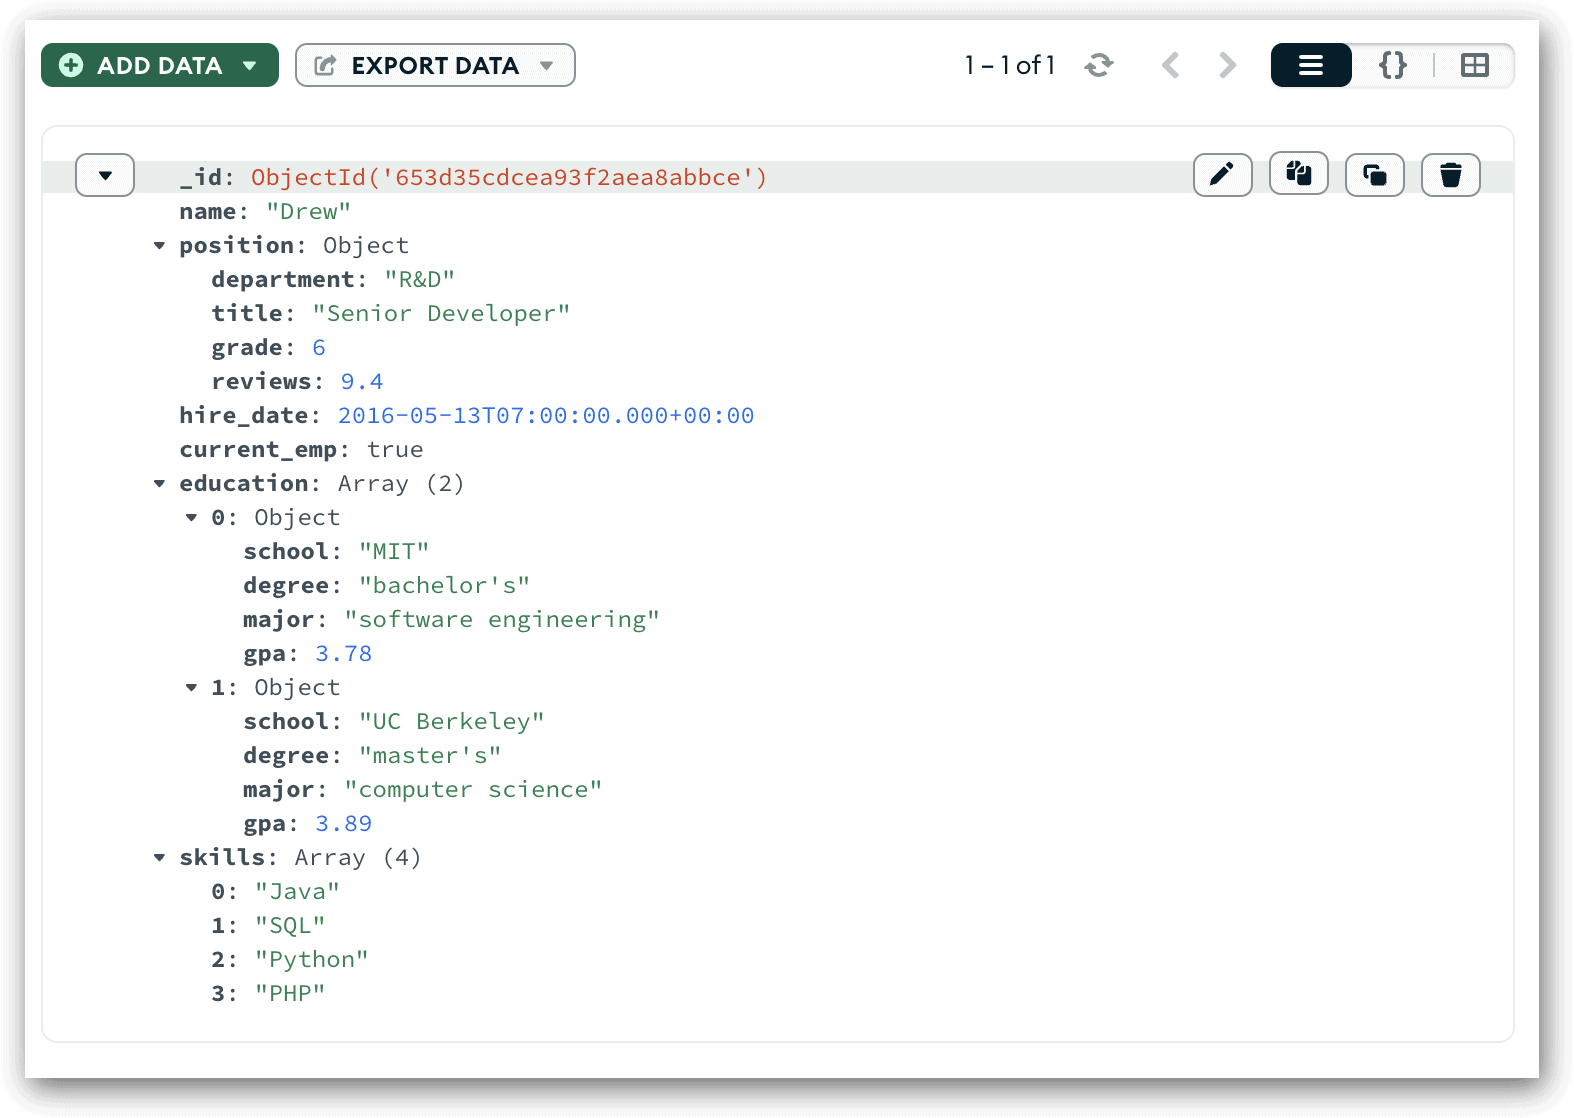
\includegraphics[width=0.75\linewidth]{images//Review_Image/MongoDB_Document.png}
    \caption{MongoDB Document Example}
    \label{fig:mde}
\end{figure}

This document encapsulates all puzzle-related information in a single, hierarchical structure.

\textbf{Schema Flexibility} $\rightarrow$ MongoDB's schema-less design allows documents in the same collection to have different structures \cite{parker2013mongodb}. This flexibility benefits chess applications where:

\begin{itemize}
    \item Different puzzle types may have \textbf{different attribute}s (endgame puzzles might include piece count, opening puzzles might reference ECO codes)
    \item New features can add fields without database \textbf{migrations}
    \item Experimental features can store \textbf{additional data }without affecting existing documents
\end{itemize}

\textbf{Indexing and Query Optimization} $\rightarrow$ MongoDB supports various index types to optimize query performance \href{https://www.mongodb.com/docs/manual/indexes/}{MongoDB Indexes}:
\begin{itemize}
    \item Single field indexes (e.g., on \texttt{difficulty})
    \item Compound indexes (e.g., on \texttt{difficulty} and \texttt{rating})
    \item Multi-key indexes for arrays (e.g., indexing \texttt{themes} array)
    \item Text indexes for full-text search
\end{itemize}

For a chess platform, indexes on \texttt{difficulty}, \texttt{themes}, and \texttt{rating} enable efficient puzzle filtering and recommendation queries.

\textbf{Aggregation Framework} $\rightarrow$ MongoDB's aggregation pipeline processes documents through multiple stages to compute analytics \href{https://www.mongodb.com/docs/manual/aggregation/}{MongoDB Aggregation}.

\subsubsection*{Comparison with Relational Alternatives}

Relational databases (PostgreSQL, MySQL) were considered but ultimately not selected:

\begin{table}[!ht]
\centering
\label{tab:db-comparison}
\newcolumntype{s}{>{\columncolor[HTML]{AAACED}} p{4cm}}
\newcolumntype{t}{>{\columncolor[HTML]{FF0000}} p{6cm}}
\newcolumntype{u}{>{\columncolor[HTML]{3CB371}} p{5.5cm}}
\begin{tabular}
{|s|t|u|}
\hline
\textbf{Aspect} & \textbf{Relational DB} & \textbf{MongoDB} \\ \hline
Schema & Fixed, requires migrations & Flexible, evolves naturally \\ \hline
Chess positions & Difficult to normalize, requires complex joins & Natural document structure \\ \hline
Querying nested data & Complex joins across tables & Simple dot notation \\ \hline
Performance for reads & Join overhead for related data & Single document retrieval \\ \hline
Development velocity & Slower due to migrations & Faster with schema flexibility \\ \hline
JSON handling & Requires ORM mapping & Native JSON/BSON \\ \hline
\end{tabular}
\caption{MongoDB vs. Relational Database Comparison}
\end{table}

For this project's requirements---flexible schema, hierarchical chess data, read-heavy workload, and rapid iteration---MongoDB's document model provides superior fit \cite{strauch2011nosql}.

\section{Development Standards}

\subsection*{REST Architectural Style}

REST (Representational State Transfer) is an architectural style for networked applications introduced by Roy Fielding in his 2000 doctoral dissertation \cite{fielding2000rest}. RESTful APIs use standard HTTP methods and conventions to perform operations on resources.

\subsubsection*{Core Principles}

\textbf{Resource-Based} $\rightarrow$ RESTful APIs organize around resources (nouns) rather than actions (verbs) \cite{rodriguez2008restful}. Resources are identified by URIs:
\begin{itemize}
    \item \texttt{/api/puzzles} represents the puzzle collection
    \item \texttt{/api/puzzles/123} represents a specific puzzle
    \item \texttt{/api/users/456} represents a specific user
\end{itemize}

\textbf{Standard HTTP Methods} $\rightarrow$ Operations on resources use standard HTTP methods with defined semantics \cite{fielding2014http}.

\textbf{Statelessness} $\rightarrow$ Each request contains all information needed for processing; no session state is stored on the server \cite{fielding2000rest}. Benefits include:
\begin{itemize}
    \item Simplified server implementation
    \item Easy horizontal scaling (any server can handle any request)
    \item Improved reliability (no session loss on server restart)
\end{itemize}

For this platform, authentication uses JWT tokens sent with each request, maintaining statelessness.

\subsubsection*{Implementation in Chess Platform}

The API follows RESTful conventions \ref{table:ras}:
\begin{table}
    \begin{tabular}{|p{3cm}|p{9cm}|}
        \hline
        \multicolumn{2}{|c|}{Puzzle endpoints} \\
        \hline
        HTTP Method & Endpoint\\
        \hline
        \hline
        GET &  \texttt{/api/puzzles?difficulty=hard\&theme=fork} \\ \hline
        POST & \texttt{/api/puzzles} \\ \hline
        GET & \texttt{/api/puzzles/:id} \\ \hline
        PUT & \texttt{/api/puzzles:id} \\ \hline
        DELETE & \texttt{/api/puzzles/:id} \\ \hline
        \hline
    \end{tabular}
    \caption{RESTful API Structure}
    \label{table:ras}
\end{table}

This design provides:
\begin{itemize}
    \item Intuitive endpoint structure
    \item Clear HTTP method semantics
    \item Easy integration with \texttt{frontend} frameworks
    \item Self-documenting API structure
\end{itemize}

\subsection*{JSON Data Format}

JSON (JavaScript Object Notation) is a lightweight, text-based data interchange format \cite{crockford2006json}. It has become the standard for web APIs, superseding XML in most modern applications.

\subsubsection*{Advantages}

\begin{enumerate}
    \item \textbf{Native JavaScript Support}: JSON parses to JavaScript objects without libraries, reducing overhead \cite{nurseitov2009json}.
    \item \textbf{Human Readable}: JSON's syntax is intuitive, facilitating debugging and manual API testing.
    \item \textbf{Compact Format}: Research by Nurseitov et al. \cite{nurseitov2009json} found JSON payloads are approximately 30\% smaller than equivalent XML, reducing bandwidth and improving load times.
    \item \textbf{Language Independent}: While based on JavaScript notation, JSON has parsers in all major programming languages \cite{ecma2017json}.
\end{enumerate}

\subsubsection*{Use in Project}

JSON is used throughout the stack:
\begin{itemize}
    \item API request and response bodies
    \item MongoDB storage (as BSON, a binary superset of JSON)
    \item Configuration files (\texttt{package.json}, \texttt{tsconfig.json})
    \item State management in React
\end{itemize}

\section{Third-Party Libraries}

\subsection*{Chess.js}

Chess.js is a JavaScript library for chess move generation, validation, and game state management \href{https://github.com/jhlywa/chess.js}{chess.js}. It provides comprehensive chess rule implementation complying with FIDE standards.

\subsection*{Key Capabilities}

\begin{itemize}
    \item \textbf{Move Generation}: Generates all legal moves for any position, accounting for checks, pins, castling rights, and en passant
    \item \textbf{Move Validation}: Ensures only legal moves are played, preventing invalid game states
    \item \textbf{FEN Support}: Loads and exports positions in Forsyth-Edwards Notation, the standard for position representation
    \item \textbf{PGN Support}: Reads and writes games in Portable Game Notation for interoperability with other chess software
    \item \textbf{Game State Detection}: Identifies check, checkmate, stalemate, threefold repetition, and fifty-move rule
    \item \textbf{Move History}: Maintains complete move history with undo capabilities
\end{itemize}

\subsubsection*{Justification}

Implementing chess rules from scratch would be error-prone and time-consuming. Chess has numerous special cases and edge conditions:

\begin{itemize}
    \item Castling (legality depends on king/rook movement history, intervening squares, check status)
    \item En passant (only legal immediately after opponent's pawn double-move)
    \item Pawn promotion
    \item Check and checkmate detection
    \item Stalemate and draw conditions
    \item Pin mechanics (pieces cannot move if doing so exposes king to check)
\end{itemize}

Chess.js provides a thoroughly tested implementation, allowing the project to focus on training features rather than rule implementation. The library has:
\begin{itemize}
    \item Over 1.3 million weekly npm downloads \href{https://www.npmjs.com/package/chess.js}{chess.js package}
    \item Comprehensive test suite
    \item Active maintenance since 2011
    \item Wide adoption in chess applications
\end{itemize}

\subsection*{React-Chessboard}

React-Chessboard is a customizable chessboard component for React applications. It provides visual board rendering with interactive piece movement \href{https://www.npmjs.com/package/react-chessboard}{react-chessboard}

\subsubsection*{Features}

\begin{itemize}
    \item \textbf{Drag-and-Drop}: Mouse and touch-based piece movement
    \item \textbf{Customization}: Configurable piece sets, board colors, and square styles
    \item \textbf{Position Control}: Accepts FEN strings for position display
    \item \textbf{Event Callbacks}: Handlers for piece drops, square clicks, and other interactions
    \item \textbf{Responsive}: Scales appropriately for different screen sizes
    \item \textbf{Accessibility}: Keyboard navigation support
\end{itemize}

\subsubsection*{Justification}

Building a chess board UI from scratch requires significant implementation effort:
\begin{itemize}
    \item SVG rendering for pieces (12 piece types with multiple design options)
    \item Drag-and-drop interaction with collision detection
    \item Touch event handling for mobile devices
    \item Responsive sizing maintaining 1:1 aspect ratio
    \item Animation for piece movements
    \item Square highlighting and annotations
\end{itemize}

React-Chessboard provides a production-ready, accessible solution, allowing focus on puzzle presentation logic, feedback mechanisms, and progress tracking rather than low-level UI implementation.

\subsection*{Authentication Libraries}

\subsubsection*{JSON Web Tokens (JWT)}

JWT (RFC 7519) is a compact, URL-safe means of representing claims between two parties \cite{jones2015jwt}. JWTs enable stateless authentication where the server doesn't maintain session storage.

\textbf{Structure:}
\begin{itemize}
    \item \textbf{Header}: Algorithm and token type
    \item \textbf{Payload}: Claims (user ID, roles, expiration)
    \item \textbf{Signature}: Cryptographic signature for verification
\end{itemize}

\textbf{Benefits for Chess Platform:}
\begin{itemize}
    \item Stateless authentication (no server session storage)
    \item Scalable across multiple servers
    \item Self-contained (includes user identity and permissions)
    \item Standard format with libraries in all languages
\end{itemize}

For user account security, bcrypt provides industry-standard password protection, ensuring that even if the database is compromised, passwords remain protected against offline attacks.

\section{Technology Stack Integration}

The selected technologies integrate to form a cohesive, modern web application architecture. Figure \ref{fig:dfde} illustrates the data flow diagram.

\begin{figure}[!ht]
    \centering
    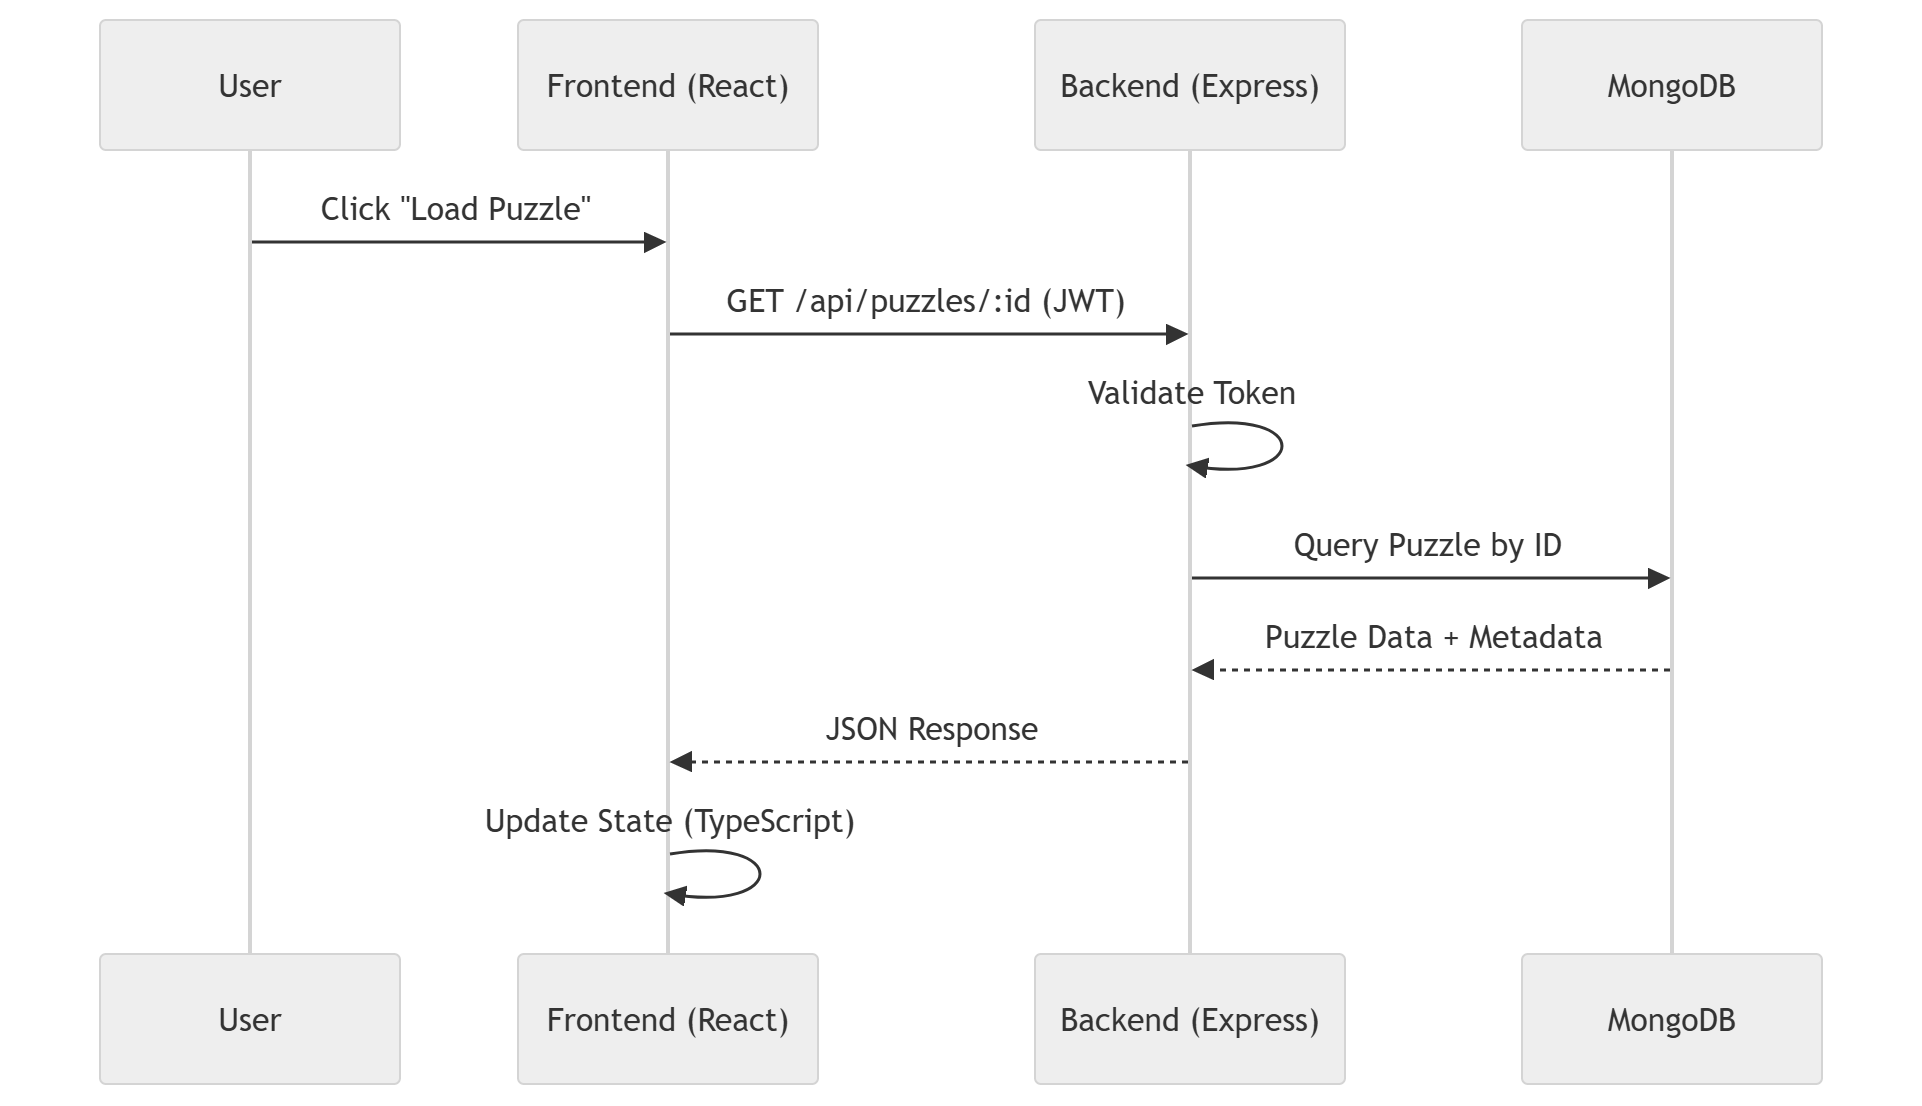
\includegraphics[width=0.75\linewidth]{images/Review_Image/DataFlow_Example.png}
    \caption{Data Flow Diagram Example}
    \label{fig:dfde}
\end{figure}

\subsection*{Data Flow Example}

A typical user interaction demonstrates technology integration:

\begin{enumerate}
    \item User clicks to load a puzzle (React component event)
    \item Frontend sends GET request to \texttt{/api/puzzles/:id} (REST, JSON)
    \item Express router receives request, validates JWT token
    \item Backend queries MongoDB for puzzle document
    \item MongoDB returns puzzle with embedded solution and metadata
    \item Backend sends JSON response to \texttt{frontend}
    \item React state updates with puzzle data (TypeScript interfaces ensure type safety)
    \item React-Chessboard renders position from FEN string
    \item User makes move via drag-and-drop
    \item Chess.js validates move legality
    \item If correct, \texttt{frontend} shows success feedback
    \item Backend receives solution attempt POST request
    \item MongoDB updates user statistics and puzzle attempt count
\end{enumerate}

This flow demonstrates seamless integration across all technology layers.

\subsection*{Technology Stack Benefits}

The integrated stack provides:

\begin{enumerate}
    \item \textbf{Performance}
    \begin{itemize}
        \item React virtual DOM optimizes rendering
        \item Node.js event loop handles concurrent users efficiently
        \item MongoDB indexes optimize puzzle queries
        \item Vite HMR accelerates development iteration
    \end{itemize}
    
    \item \textbf{Scalability}
    \begin{itemize}
        \item Stateless REST API enables horizontal scaling
        \item MongoDB supports sharding for data distribution
        \item JWT authentication requires no server-side session storage
    \end{itemize}
    
    \item \textbf{Maintainability}
    \begin{itemize}
        \item TypeScript catches errors at compile-time
        \item Component architecture promotes code reuse
        \item Clear separation of concerns (frontend/backend/database)
        \item Shared JavaScript enables code reuse across stack
    \end{itemize}
    
    \item \textbf{Developer Experience}
    \begin{itemize}
        \item Single language (JavaScript/TypeScript) across stack
        \item Rich ecosystem of libraries and tools
        \item Excellent IDE support with autocomplete and type checking
        \item Fast development feedback loops
    \end{itemize}
\end{enumerate}

\section*{Conclusion}

This technology review has examined the complete technology stack for ``Guardians of the Chess Grandmaster,'' demonstrating thorough research and justified selection based on project requirements, performance characteristics, and academic literature.

The chosen stack---React with TypeScript for \texttt{frontend}, Node.js with Express for \texttt{backend}, and MongoDB for database---provides a robust, modern foundation for building a chess training platform that meets the objectives outlined in the introduction:

\begin{itemize}
    \item \textbf{Interactive Training}: React and React-Chessboard enable smooth, responsive board interactions
    \item \textbf{Real-Time Feedback}: Chess.js provides instant move validation
    \item \textbf{Progress Tracking}: MongoDB's flexible schema accommodates evolving user statistics
    \item \textbf{Cross-Device Support}: Responsive React components and mobile-friendly design
    \item \textbf{Scalability}: Stateless architecture and efficient I/O handling support growth
\end{itemize}

Each technology selection was justified through:
\begin{itemize}
    \item Alignment with project-specific requirements
    \item Performance characteristics relevant to chess applications
    \item Industry adoption and community support
    \item Academic research demonstrating effectiveness
    \item Standards compliance ensuring interoperability
\end{itemize}

The technology review establishes the technical foundation upon which subsequent chapters build system design, implementation details, and evaluation. The selection of mature, well-documented, industry-standard technologies minimizes technical risk while providing the flexibility needed for iterative development and future feature enhancement.